% =====================================
% Purpose: Create a Robert Bringhurst style thesis paper using the 
% classicthesis package and some custom enhancements - this is 
% the default template for most of my documents
% =====================================

% =====================================
% Document Class and main packages
% =====================================

\documentclass[10pt,a4paper, hidelinks]{article} % KOMA-Script article scrartcl
\usepackage[nochapters, pdfspacing]{classicthesis} % [nochapters] [drafting] (puts date/time at bottom) [beramono] (changed mono spaced font)

% =====================================
% Packages in Use
% =====================================

%Math Packages
\usepackage{amsmath}
\usepackage{amsfonts}
\usepackage{amssymb}
\usepackage{nicefrac} % For typsetting inline fractions
\usepackage{mathtools} % For substack and mathclap (underbrace helper commands)

%% Typography enhancements
\usepackage{microtype} % For awesome typographical improvements
\usepackage{booktabs} % Pretty \begin{tabular}
\usepackage{multicol} % For pretty multi-columns enviroments
\usepackage{xspace} % For use in a command to ensure proper spacing
%\usepackage{geometry} %uncomment this is you want full page documentation
\usepackage{graphicx} % for allowing pictures
\usepackage{float} % For the purpose of adding \begin{figure} [H]
\usepackage{lipsum} % For adding filler text
\usepackage{wasysym} % For the \newmoon command for the legal blobs

% For commenting on incomplete or new items
\usepackage{todonotes} % \missingfigure{} is the best command

% For inclusion of PDFs in the document \includepdf[pages={3,{},8-11,15}]{example.pdf}
% This will include page 3, a blank page, 8,9,10,11, and 15
% you can set this to draft to get boxes or final to get the default which includes
% the pages
% Options:
% 	fitpaper: Use this to insert the page as is - otherwise items are scaled to page
% 	rotateoversize: Attempt to rotate oversized pages and scale them
\usepackage[final]{pdfpages}

% =====================================
% Graphics 
% =====================================

% For quick graphics insert -- Full Line --
\newcommand{\qpic}[2]{
\begin{figure}[H]
\centering
\includegraphics[width=1\linewidth]{./#1}
\caption{#2}
\label{fig:#1}
\end{figure}
}

% For quick graphics insert -- Normal Size --
\newcommand{\qpics}[2]{
\begin{figure}[H]
\centering
\includegraphics[width=0.7\linewidth]{./#1}
\caption{#2}
\label{fig:#1}
\end{figure}
}

% =====================================
% Custom Macros that make life easier
% =====================================

% Description Enviroment Item Helper Commands
\newcommand{\im}[1]{\item[#1] \xspace}
\newcommand{\imp}[1]{\item[(#1)] \xspace}

% Auto-commas for long nominal and dollar amounts
\RequirePackage{siunitx}
\newcommand{\commasep}[1]{\num[group-separator={,}]{#1}}
\newcommand{\money}[1]{\$\commasep{#1}}

% Borrowing from tufte, this is the \newthought command that is 
% often used to bring about the change from one subsubsection
% to another and is a good way to bring things up logically into smaller
% bites
\newcommand{\newthought}[1]{
\vspace{11pt} \noindent
\spacedlowsmallcaps{#1}
}

% Code for the fast creation of bullet lists
\newcommand{\qb}[1]{\begin{itemize} #1 \end{itemize}}

% Code to produce spaced small caps in real text
\newcommand{\mysmallcaps}[1]{\spacedlowsmallcaps{#1}\xspace}

% Legal blobbing for reminding oneself to include information there: [<circle>]
\newcommand{\legalblob}{\ensuremath{\left[\newmoon\right]}}

% Simple math macros for probablility and expectations that are very common for math homework
\newcommand{\p}{\ensuremath{\mathbb{P}}\xspace}
\newcommand{\expt}[1]{\ensuremath{\mathbb{E}}\left[#1\right]\xspace}
\newcommand{\myvec}[1]{\underset{\sim}{#1}}
\newcommand{\myexp}[1]{\exp\left( #1\right) }

% =====================================
% For handling code blocks and other text
% =====================================

% Code to handle inputting code segments in R
% To import code use: \lstinputlisting[language=R]{h1code.r}
% To add code in-line use \begin{lstlisting}[language = {}] 
% \lstinputlisting[language={}]{file.txt} for  unformatted code
\usepackage{listings} 
\lstset{language=R} 
\usepackage{color}
\definecolor{mygreen}{rgb}{0,0.6,0}
\definecolor{mygray}{rgb}{0.5,0.5,0.5}
\definecolor{mymauve}{rgb}{0.58,0,0.82}

\lstset{ %
  backgroundcolor=\color{white},   % choose the background color; you must add \usepackage{color} or \usepackage{xcolor}
  basicstyle=\footnotesize,        % the size of the fonts that are used for the code
  breakatwhitespace=false,         % sets if automatic breaks should only happen at whitespace
  breaklines=true,                 % sets automatic line breaking
  captionpos=b,                    % sets the caption-position to bottom
  commentstyle=\color{mygreen},    % comment style
  deletekeywords={...},            % if you want to delete keywords from the given language
  escapeinside={\%*}{*)},          % if you want to add LaTeX within your code
  extendedchars=true,              % lets you use non-ASCII characters; for 8-bits encodings only, does not work with UTF-8
  frame=single,	                   % adds a frame around the code
  keepspaces=true,                 % keeps spaces in text, useful for keeping indentation of code (possibly needs columns=flexible)
  keywordstyle=\color{blue},       % keyword style
  language=R,                 % the language of the code
  otherkeywords={*,...},            % if you want to add more keywords to the set
  numbers=left,                    % where to put the line-numbers; possible values are (none, left, right)
  numbersep=5pt,                   % how far the line-numbers are from the code
  numberstyle=\tiny\color{mygray}, % the style that is used for the line-numbers
  rulecolor=\color{black},         % if not set, the frame-color may be changed on line-breaks within not-black text (e.g. comments (green here))
  showspaces=false,                % show spaces everywhere adding particular underscores; it overrides 'showstringspaces'
  showstringspaces=false,          % underline spaces within strings only
  showtabs=false,                  % show tabs within strings adding particular underscores
  stepnumber=2,                    % the step between two line-numbers. If it's 1, each line will be numbered
  stringstyle=\color{mymauve},     % string literal style
  tabsize=2,	                   % sets default tabsize to 2 spaces
  title=\lstname                   % show the filename of files included with \lstinputlisting; also try caption instead of title
}

% =====================================
% Beginning the main document
% =====================================

\begin{document}
\pagestyle{plain} 
\title{\rmfamily\normalfont\spacedallcaps{Learning the Madness - NCAA March Madness Predictions}}
\author{\spacedlowsmallcaps{Andrei Kopelevich $\bullet$ Mark Kurzeja $\bullet$ Eli Schultz }}
\date{} % no date or \today if you want to insert a date

\maketitle

\begin{abstract}
	Every year, millions of people fill out March Madness brackets in attempt to predict the outcome of the NCAA men's basketball tournament. A big part of the draw is that the tournament is notoriously difficult to predict, and predicting a perfect bracket is so improbable that Warren Buffet, a US investor, annually offers \$1MM a year for life to any of his employees who can predict the exact outcome of the tournament. Many algorithms for predicting the tournament attempt to predict results at the individual game level, based on how teams match up with one another. We will instead focus on predicting how many rounds a team will progress in the tournament based on its performance over the course of the preceding season, with the goal of building stable predictions and successfully predicting tournament outcomes.
\end{abstract}

\tableofcontents
\newpage

\section{Background}
After all regularly scheduled NCAA basketball games are concluded in mid-March, 68 teams are selected to participate in the NCAA tournament. Every game is single elimination, meaning that as soon as a team loses it is eliminated from the tournament. Eight of the 68 teams originally chosen have to compete in so-called play-in games, after which 64 teams remain. We will follow the same framework as that followed by most bracket prediction contests and concern ourselves here with predicting how teams will perform once the field has been narrowed down to 64 contenders. At this point there are $2^{32} \cdot 2^{16} \cdot 2^8 \cdot 2^4 \cdot 2^2 \cdot 2 = 2^{63}$ possible outcomes, which gives one an idea of the scope of this challenge. Predicting a perfect bracket may be impossible, but we will see how close we can get.

The first step in our analysis was gathering data. There are many decades of team performance data available on the Sports Reference college basketball website free of charge. However, in recent years a number of more advanced metrics have been devised that have been shown to more accurately capture a team's strength. Since this data is only available starting from 1993, we limited our analysis to that timeframe. Our working data set ultimately consisted of 12 continuous quantitative predictors, and one categorical response corresponding to the number of victories a team had in the tournament (ranging from 0 for a team that lost immediately to 6 for a national champion).

The predictors can be thought of as belonging to six broad buckets corresponding to aspects of a team performance:

\begin{itemize}
	\item Winning percentage, strength of schedule (SOS) and simple rating system (SRS) are all holistic measures.
	\item Free throw attempt rate (ft\_rate0), free throw attempts per field goal attempt (fta\_per\_fga\_pct), and three-point attempts per field goal attempt (fg3a\_per\_fga\_pct), and assist rate (ast\_pct) all help classify a team's offensive playing style. The idea is that three-point shots are high risk and high reward while free throws are low risk and low reward. Thus teams that attempt more three point shots may have more variable performances from game to game, while teams that attempt more free throws may be more consistent. Teams with higher assist rates should be expected to play more collaboratively, while teams with low assist rates rely more on strong individual performances.
	\item Total rebound percentage (trb\_pct) captures how well a team recovers the ball following shots missed by either themselves or their opponents.
	\item True shooting percentage (ts\_pct) and effective field goal percentage (efg\_pct) both capture how well a team shoots the ball.
	\item Turnover percentage (tov\_pct) captures how well a team is able to avoid allowing the other team to take the ball away (better teams should generally have lower turnover percentages).
	\item Block percentage (blk\_pct)  captures how well a team is able to block the other team's shots.
\end{itemize}

It is worth noting that the vast majority of these statistics capture how well a team performs offensively.  

\section{Preliminary Data Exploration}

\subsection{Data Exploration and Visualization}
We began by performing data exploration and visualization, as well as dimension reduction, to inform our analysis.

Summaries of the predictors are provided below.

\missingfigure{SUMMARY}

At a high level, the first three predictors provide a good sanity check in that they suggest that  teams in the tournament are generally better than average teams. The first quartile for winning percentage (percentage of games that a given team won) is well above 50\% for the teams in our data set. Our teams also generally have strength of schedule and simple rating system scores well above zero, which is to be expected given that those metrics are designed such that an average team will have a score around zero. It may seem a bit strange at first that stronger teams will tend to have a better SOS score, but this can be explained by the fact that strong teams tend to be in the same conferences as other strong teams, and therefore play other strong teams more frequently.

It is also worth noting that a number of the predictors have unusually large and/or small outliers. To visualize high-level trends in the predictors, boxplots of each of the predictors for each of the six tournament win groups are provided below. Some of the predictors, such as assist percentage and the two free-throw related predictors, seem to be fairly similarly distributed across the six groups. However, there are a number of pronounced patterns. For instance, more successful tournament teams generally tend to much higher win-loss percentages, SRS, and SOS scores. This is also true, although to a lesser extent for true shooting percentage, effective field goal percentage, total rebound percentage, and block percentage. Similarly, more successful teams tend to have lower turnover rates. 

\begin{figure}[H]
	\centering
	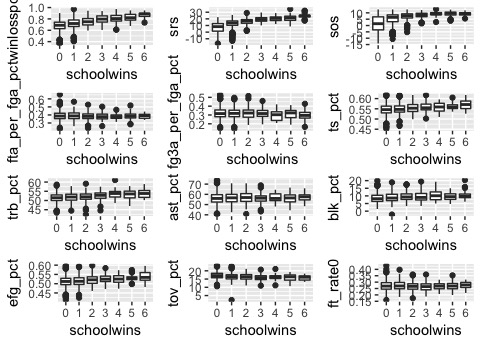
\includegraphics[width=0.7\linewidth]{../fig/RayleighWetDream}
	\caption{caption goes here}
	\label{fig:rayleighwetdream}
\end{figure}


A pairwise scatterplot of the predictors is provided below. Many of the correlations are relatively small. Unsurprisingly, in some cases where two predictors belong to the same bucket (per the framework above) we notice very strong correlations. Effective field goal percentage and true shooting percentage are the most strongly correlated predictors ($r \approx 0.96$), which is to be expected given that both measure how well a team shoots the ball. Free throw rate and free throw attempts per field goal attempt ($r \approx 0.922$) both capture how often a team tends to shoot free throws in slightly different ways. Finally, the strong correlations between SRS and wining percentage ($r \approx 0.518$) and SRS and SOS ($r \approx 0.867$) reflect the fact that SRS is meant to capture team performance, adjusted for strength of schedule.

\begin{figure}[H]
	\centering
	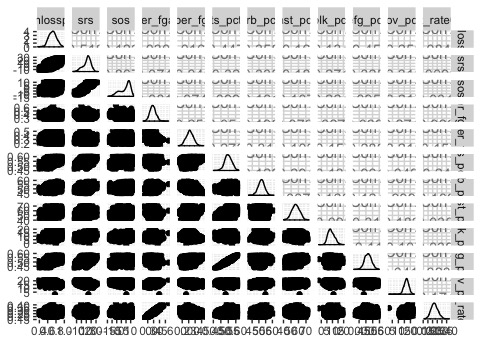
\includegraphics[width=0.7\linewidth]{../fig/MoneyMaker}
	\caption{caption goes here}
	\label{fig:ggpairs}
\end{figure} 

However, there are a few other correlations that are much weaker, but perhaps a little more interesting conceptually. For instance, there is a weak negative correlation between rebounding percentage and free throw attempts per field goal attempt ($r \approx -0.311$), a correlation which does not seem to have an obvious intuitive explanation based on the buckets outlined above. Similarly, both true shooting percentage ($r \approx 0.273$) and effective field goal percentage ($r \approx 0.282$) were weakly correlated with three point attempts per field goal attempt.

Overall, the presence of these correlations suggests that it may be useful to perform PCA in an attempt to reduce overall dimensionality.

A skree plot of percentage of variance explained against number of principal components used is shown below. 

\missingfigure{Skreeeeee}

The data projected onto the first two principal components, which only explain about 44\% of the variability within the data set, appear as follows:

\begin{figure}[H]
	\centering
	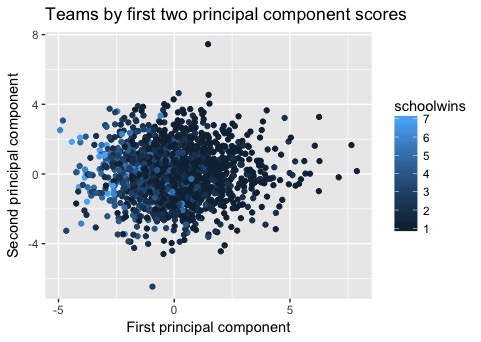
\includegraphics[width=0.7\linewidth]{../fig/PrinComps}
	\caption{caption goes here}
	\label{fig:princomps}
\end{figure}


While we do not necessarily observe perfect clustering corresponding to each of the possible win totals, it is encouraging to see that the first principal component in particular seems to do a fairly good job of differentiating weak teams from strong ones, with teams that advanced further in the tournament tending to have lower scores for that component. Although this trend is much less pronounced, it appears that stronger teams may also tend to have slightly higher scores for the second principal component. 


\subsection{Ordinal Regression}

When looking at our problem, we ran into an issue with the domain of the response variable - the number of rounds that a given team will make it in the tournament. In particular, our response variable is neither continuous (since it takes on only integer values and is bounded), nor is this a pure classification problem (because their is a natural ordering in the response). As a result, we need to run an ordinal regression, at least in the onset, and see how well the data can be summarized with these approaches before we can move onto more complicated models. 

For the ordinal regression problem, we chose to use the \texttt{rstanarm polr} functions, as this allows us to view the posterior distributions of the coefficients, and determine if any of the coefficients are significant. In order to see the relative effect, we begin by standardizing the variables as well as centering them. Otherwise, the coefficients will not be on the same unit scale and we want to avoid this in our analysis. We begin by excluding the teams names themselves to see if the other predictor variables can be used to discern performance. 

We run the checks on the posterior distribution, and see that each of the four chains used have, indeed, converged, there was no divergences in any of the four chains, and the tree-depth was not hit on any of the iterations signaling that the prior distribution on $R^2$ was sufficiently informative enough to ensure that the chains did not explore too distant from the true posterior distribution. For information on how the prior distribution is set up or on the operation of \texttt{rstanarm}, please refer to the guide here: {\color{blue} \url{https://cran.r-project.org/web/packages/rstanarm/rstanarm.pdf}}

The posterior distributions for the log-odds of the parameters are as follows:

% latex table generated in R 3.4.3 by xtable 1.8-2 package
% Sat Apr 07 15:09:49 2018
\begin{table}[ht]
	\centering
	\begin{tabular}{lrrrrrrr}
		\toprule
		Parameter & Rhat & n\_eff & mean & sd & 2.5\% & 50\% & 97.5\% \\ 
		\midrule
		games & 1.0 & 1400 & 3.1 & 6.8 & -8.4 & 2.5 & 18.0 \\ 
		overallwins & 1.0 & 1403 & -3.5 & 11.3 & -28.4 & -2.6 & 15.7 \\ 
		overalllosses & 1.0 & 1402 & -3.5 & 8.4 & -21.6 & -2.7 & 10.9 \\ 
		winlosspct & 1.0 & 2000 & -0.4 & 0.7 & -1.7 & -0.4 & 1.0 \\ 
		srs & 1.0 & 2000 & 0.8 & 0.5 & -0.1 & 0.8 & 1.8 \\ 
		sos & 1.0 & 2000 & 0.2 & 0.4 & -0.5 & 0.2 & 0.9 \\ 
		wins\_conf & 1.0 & 2000 & -0.2 & 0.1 & -0.4 & -0.2 & -0.1 \\ 
		losses\_conf & 1.0 & 2000 & -0.3 & 0.1 & -0.5 & -0.3 & -0.1 \\ 
		pts & 1.0 & 2000 & -0.4 & 0.5 & -1.3 & -0.4 & 0.5 \\ 
		opp\_pts & 1.0 & 2000 & 0.5 & 0.4 & -0.2 & 0.5 & 1.2 \\ 
		fta\_per\_fga\_pct & 1.0 & 2000 & 1.0 & 0.7 & -0.4 & 1.0 & 2.3 \\ 
		fg3a\_per\_fga\_pct & 1.0 & 2000 & -0.1 & 0.1 & -0.2 & -0.1 & 0.0 \\ 
		ts\_pct & 1.0 & 2000 & 2.3 & 1.5 & -0.7 & 2.3 & 5.2 \\ 
		trb\_pct & 1.0 & 2000 & -0.1 & 0.1 & -0.2 & -0.1 & 0.0 \\ 
		ast\_pct & 1.0 & 2000 & -0.0 & 0.1 & -0.1 & -0.0 & 0.1 \\ 
		blk\_pct & 1.0 & 2000 & -0.1 & 0.0 & -0.2 & -0.1 & -0.1 \\ 
		efg\_pct & 1.0 & 2000 & -2.2 & 1.4 & -4.9 & -2.2 & 0.5 \\ 
		tov\_pct & 1.0 & 2000 & 0.2 & 0.1 & 0.1 & 0.2 & 0.3 \\ 
		ft\_rate0 & 1.0 & 2000 & -1.5 & 1.0 & -3.3 & -1.5 & 0.4 \\ 
%		0$|$1 & 1.0 & 2000 & -0.2 & 0.1 & -0.3 & -0.2 & -0.0 \\ 
%		1$|$2 & 1.0 & 2000 & 1.5 & 0.1 & 1.4 & 1.5 & 1.7 \\ 
%		2$|$3 & 1.0 & 2000 & 2.8 & 0.1 & 2.6 & 2.8 & 3.0 \\ 
%		3$|$4 & 1.0 & 2000 & 3.9 & 0.1 & 3.6 & 3.9 & 4.2 \\ 
%		4$|$5 & 1.0 & 2000 & 4.8 & 0.2 & 4.4 & 4.8 & 5.2 \\ 
%		5$|$6 & 1.0 & 2000 & 5.7 & 0.2 & 5.3 & 5.7 & 6.2 \\ 
%		mean\_PPD:0 & 1.0 & 2000 & 0.5 & 0.0 & 0.4 & 0.5 & 0.5 \\ 
%		mean\_PPD:1 & 1.0 & 2000 & 0.3 & 0.0 & 0.2 & 0.3 & 0.3 \\ 
%		mean\_PPD:2 & 1.0 & 2000 & 0.1 & 0.0 & 0.1 & 0.1 & 0.2 \\ 
%		mean\_PPD:3 & 1.0 & 2000 & 0.1 & 0.0 & 0.0 & 0.1 & 0.1 \\ 
%		mean\_PPD:4 & 1.0 & 2000 & 0.0 & 0.0 & 0.0 & 0.0 & 0.0 \\ 
%		mean\_PPD:5 & 1.0 & 2000 & 0.0 & 0.0 & 0.0 & 0.0 & 0.0 \\ 
%		mean\_PPD:6 & 1.0 & 2000 & 0.0 & 0.0 & 0.0 & 0.0 & 0.0 \\ 
%		log-posterior & 1.0 & 438 & -1770.7 & 4.7 & -1780.6 & -1770.3 & -1762.4 \\ 
		\bottomrule
	\end{tabular}
\end{table}

\missingfigure{Don't forget that when intrepreting the log-odds that R reverses the sign compared to other programs. Look here for the math: \url{https://stats.stackexchange.com/questions/89474/interpretation-of-ordinal-logistic-regression}}

We need to note that the coefficients do not have the most meaningful interpretations, but since they are all standardized, we can use their absolute magnitude and whether their credible intervals contain zero to discern their relevance. If a given credible interval contains zero, we can say that it is reasonably likely that the $\exp(\beta_i) = 1$ which indicates that their is reason to believe that the odds ratio can be one. This is equivalent to saying that there is no significant change in the odds with the use of this coefficient. 

We first aim to explain why the variances of the \texttt{games}, \texttt{overallwins}, and \texttt{overalllosses} variables have such high variance relative to the other variables. To see this, we will plot the ggpairs plot of the posteriors to determine what is going on.

\begin{figure}[H]
	\centering
	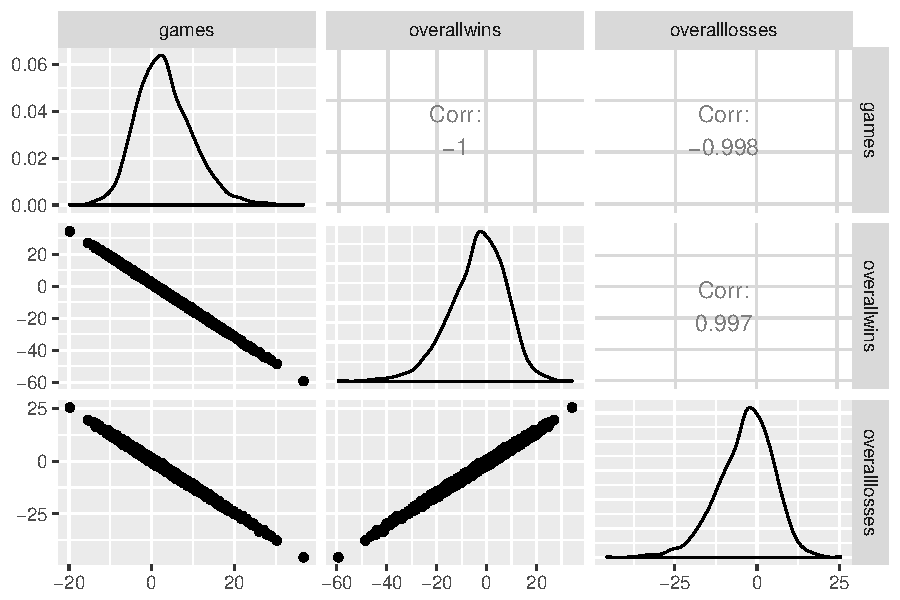
\includegraphics[width=0.7\linewidth]{../fig/polr_correlation}
	\caption{We can see that games, overallwins, and overall losses are highly correlated with one another. As a result, we are getting a case of the "bouncing betas" that we encounter in simple linear regression - this is something that we should account for because the coefficients are basically fighting one another for significance in the model and we have a high amount of collinearity. When we look at the model, we see that games correlates highly with overall wins and overall wins correlates highly with overall losses.}
	\label{fig:polrcorrelation}
\end{figure}

We also see that there are some pretty strong correlations between the effective field goal percentage, total shooting percentage, and other variables. We aim to reduce the multi-collinearity in the model by removing those terms that have significant correlation with one another, and then we refit the model. 


The in-sample performance of the Bayesian regression method is given by the following 7x7 confusion matrix (the left column is the true values and the top row is the predicted values):
\begin{figure}[H]
	\centering
	% latex table generated in R 3.4.3 by xtable 1.8-2 package
	% Sun Apr 08 14:53:18 2018
		\begin{tabular}{r|cccccc}
			\toprule
			& 0 & 1 & 2 & 3 & 4 & 6 \\ 
			\midrule
			0 & 685 &  89 &   0 &   0 &   0 &   0 \\ 
			1 & 215 & 178 &  15 &   0 &   1 &   0 \\ 
			2 &  43 & 116 &  29 &   5 &   0 &   0 \\ 
			3 &   1 &  46 &  35 &  16 &   0 &   0 \\ 
			4 &   0 &   9 &  23 &  13 &   1 &   1 \\ 
			5 &   0 &   3 &   5 &  11 &   1 &   5 \\ 
			6 &   0 &   0 &   4 &  12 &   4 &   4 \\ 
			\bottomrule
		\end{tabular}
\caption{We can see that the algorithm is good at separating out the first round losers given that it only incorrectly classifies 89 of the teams that lost in the first round as going onto the second round. As we get into the middle rounds, however, we can see that it is much harder to classify correctly, and the regression downward biases the results - we can see that of those that make it to the fourth round, it has terrible performance at predicting that is the case. Similarity, it does not predict that anyone would make the fifth round which is troublesome considering that by the design of the tournament $4/64$ of the teams make it to the final four. This shows us that the data is just very difficult to work with, and that it is very noisy even in sample. March is, indeed, Mad.}
\end{figure}


We begin by looking for those coefficients that do not contain zero in their confidence interval
\missingfigure{This needs to be updated now that the algo has been rerun}
\begin{description}
	\item[wins\_conf] We can see that the wins number inter-conference has a negative coefficient but the magnitude of the coefficient does not indicate that it is practically significant as the odds of changing levels in the tournament are only affected by about  22\% ($\exp(-0.1) \approx 1.22$) (positivity). Since the odds are increasing, this indicates that teams that tend to play and win more conference games tend to do better in the tournament. This result makes sense. 
	\item[loses\_conf] The mean of this term is, like the wins\_conf pretty insignificant from a practical standpoint as it only increases the odds by about 34\% ($\exp(.34) = 1.33$). The sign of this coefficient seems to be counter intuitive as we would expect the wins to have a positive effect on the odds and the losses to have a negative effect on the odds. I think that the fact that the increase in odds for these variables indicate that those teams that tend to play a larger number of games than their opponents during the season tend to do better in the tournament. This could makes sense as schools that are smaller tend to do worse in the tournament.  
	\item[blk\_pct] Accounting for the blocking percentage, this tells us that for every standard deviation that a team blocks above the average, the odds of them winning increase by about 10\% which is in line with our intuition. Given how devastating certain blocks can be to the psyche of the other team, and how critical often a few points are in the tournament, the ability to block is a feature that we expected to be critical to the performance of a team.
\end{description}








\begin{figure}[H]
	\centering
	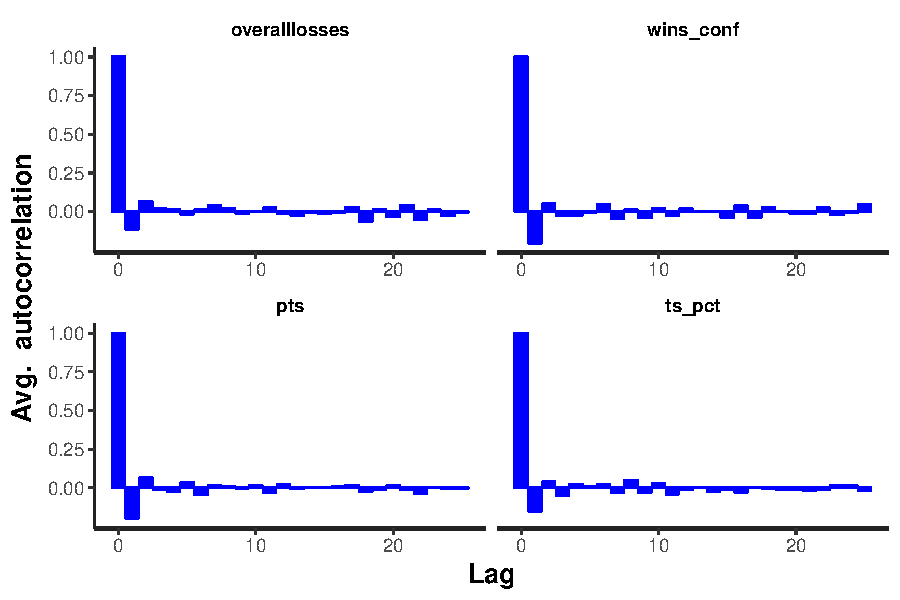
\includegraphics[width=1\linewidth]{../fig/polr_autocorr}
	\caption{The autocorrelation on all of the parameters looked similar to the auto-correlation above - we can see that the posterior was explored throughly and the chains did not get stuck for long in any one particular area. }
	\label{fig:polr_autocorrelation}
\end{figure}

%\begin{figure}
%	\centering
%	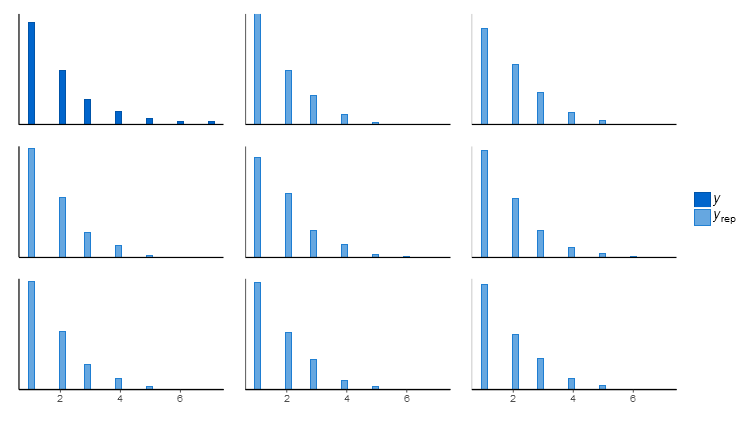
\includegraphics[width=1\linewidth]{../fig/polr_pp}
%	\caption{The upper left histogram is the true distribution of the factor levels of $y$. We can see that their are seven levels - each one half the size of the preceding bar since a team either makes it or does not make it to the next round. We can see that the posterior predictive distributions more or less seem to capture this well, but we can see that for levels greater than four (i.e. for teams that made it to the final four) the ordinal regression model fails to predict well in these tails. As a result, this may be something that we need to correct for when looking at the final four contenders.}
%	\label{fig:polr_pp}
%\end{figure}

\begin{figure}[H]
	\centering
	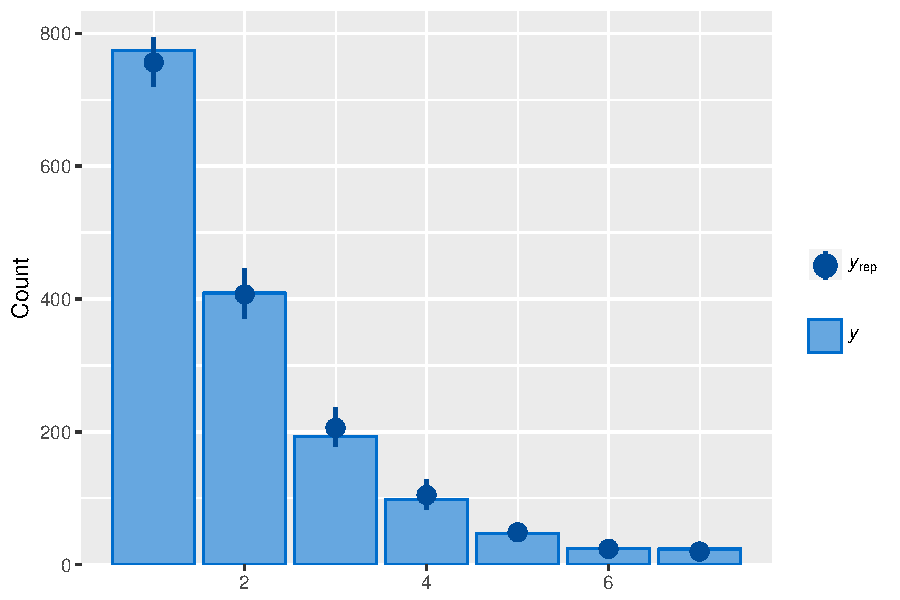
\includegraphics[width=0.7\linewidth]{../fig/polr_nonames_pp}
	\caption{This is a summary of the posterior predictive distribution for the first model that we have run with ordinal regression. We can see that the posterior is one of seven counts, we can see that if we run simulation from the predictive posterior, the counts that we get are right in line with what we observed. This indicates that the model is capturing the frequency of the counts in its inference which is important if we are not going to under bias or over bias any particular outcome. We can see that, especially at $wins = 0$, that the count is bias downwards however. We will fit a more complicated model that takes into teams individual performance shortly which will hopefully fix this bias.}
	\label{fig:polrnonamespp}
\end{figure}



\begin{figure}[H]
	\centering
	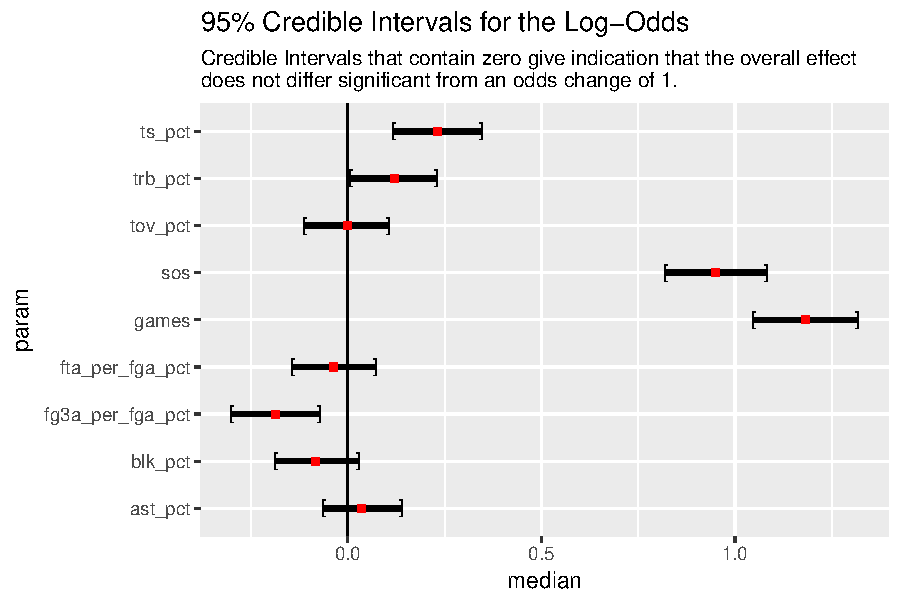
\includegraphics[width=1\linewidth]{../fig/polr_coef}
	\caption{replace this with the ggplot version saved down}
	\label{fig:polr_coef}
\end{figure}

\begin{figure}[H]
	\centering
	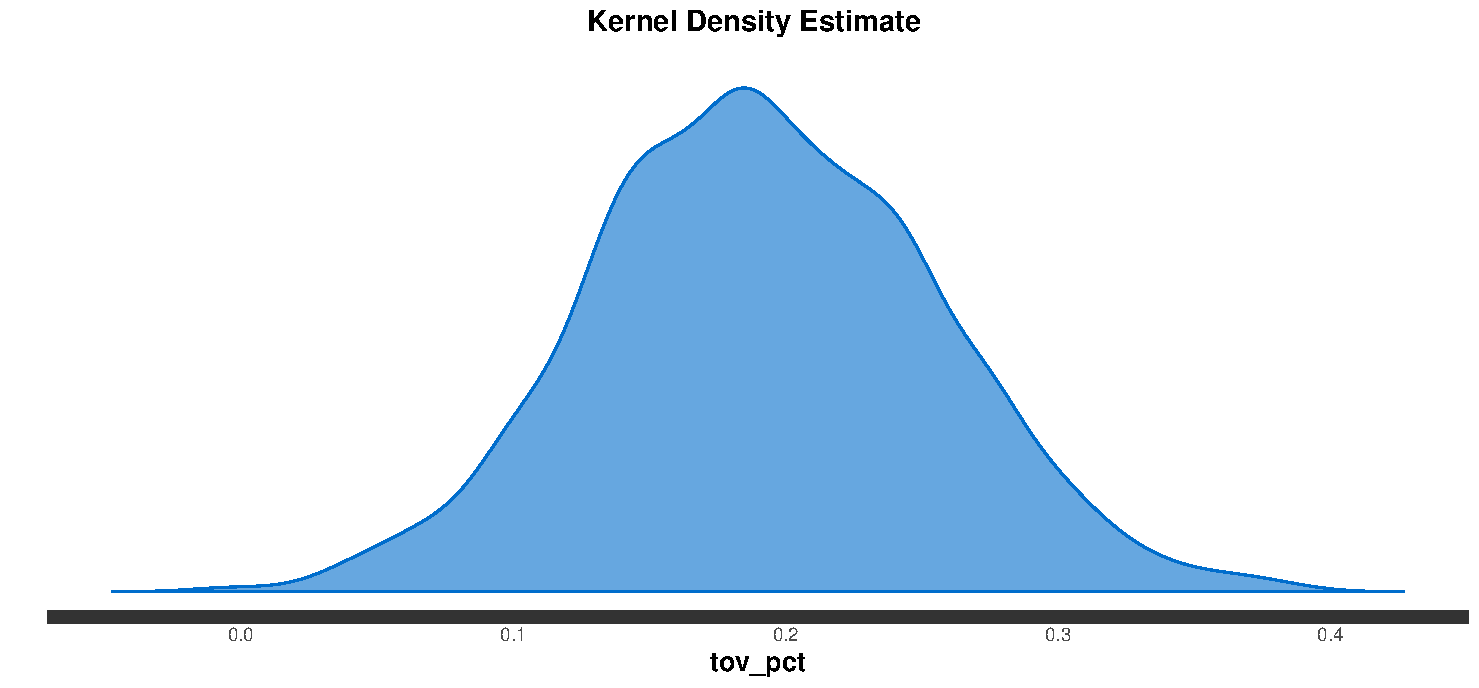
\includegraphics[width=0.7\linewidth]{../fig/polr_tovpct}
	\caption{The turn-over percentage(tov\_pct) has a positive coefficient which makes sense in the context of the problem. For every standard deviation that a team turns over the ball more than the field on average, we see about a 19\% change in the odds that they lose. This is significant and is in-line with intuition that turnovers can be the critical factor in a tight game in the tournament}
	\label{fig:polrtovpct}
\end{figure}

\begin{figure}[H]
	\centering
	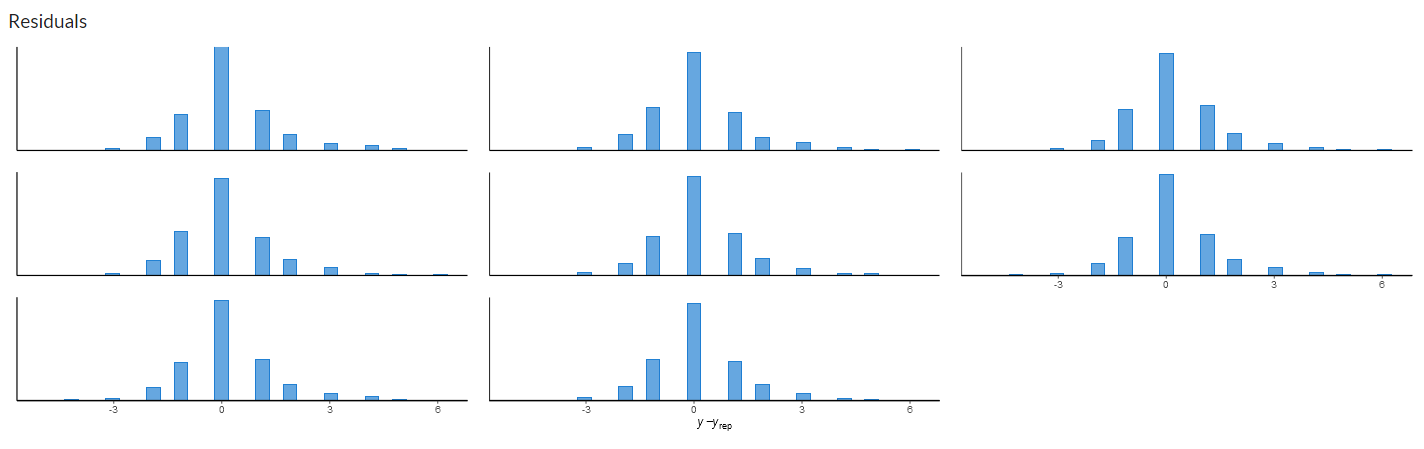
\includegraphics[width=1\linewidth]{../fig/polr_residuals}
	\caption{captionhere}
	\label{fig:residuals}
\end{figure}

\missingfigure{Still under construction :) - include the results of working with the names model}

\begin{figure}[H]
	\centering
	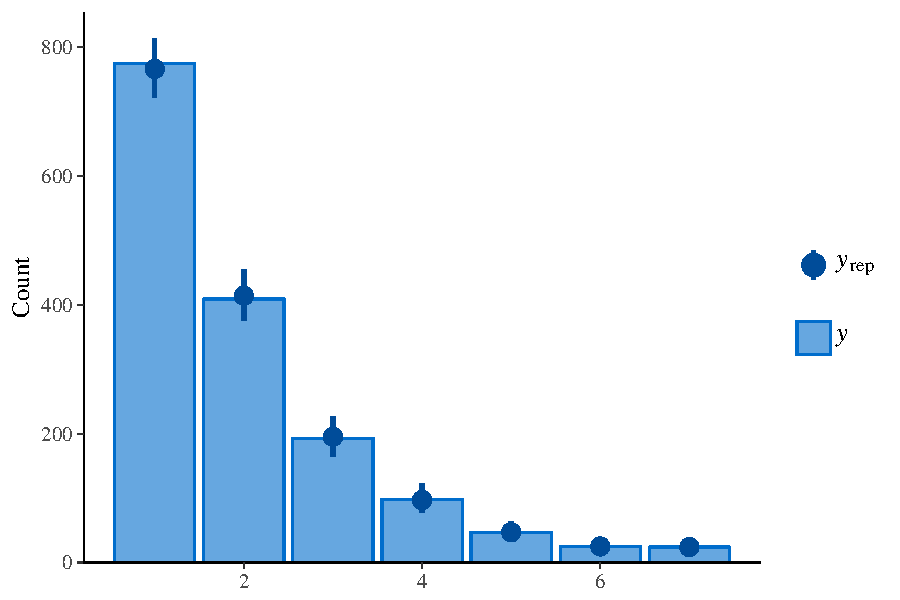
\includegraphics[width=0.7\linewidth]{../fig/polr_name_pp}
	\caption{If we include the names as variables, we can see that the posterior predictive distribution frequency count is almost spot on with what we observe. This makes sense that our predictions would get better accounting for the individual team variability in the model, but we need to find out if the prediction that comes from this model is something that outperforms the simpler model and is not bias downwards on the predictions of how many people are going to make the tournament, but it is not a drastically improved fit.}
	\label{fig:polrnamepp}
\end{figure}

\begin{figure}[H]
	\centering
	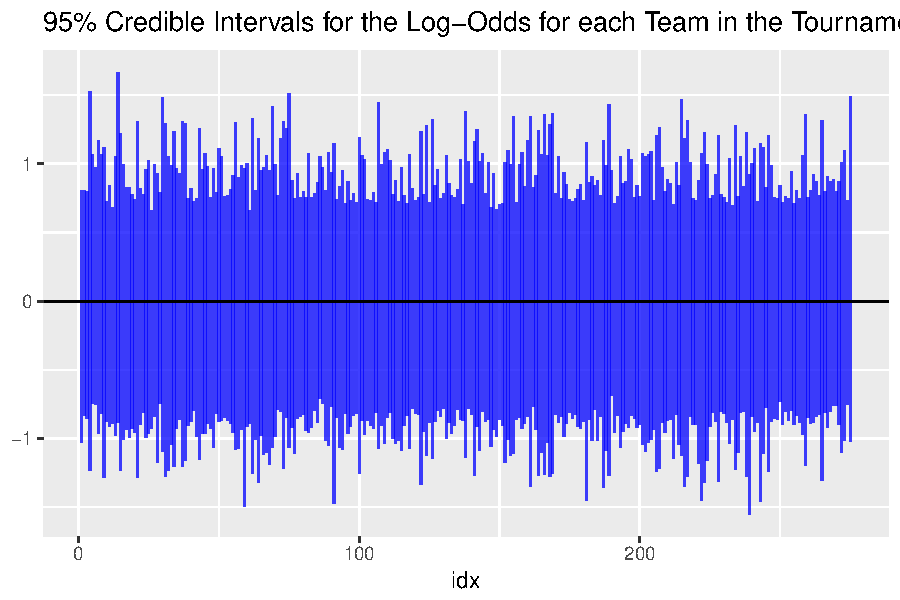
\includegraphics[width=0.7\linewidth]{../fig/polr_team_log_odds}
	\caption{We can see that the 95\% posterior interval for each of the teams is centered around, and contains zero. This is an indication that for no team in the tournament does their name, controlling for things like shooting percentage performance, account for over or under performance. This finding was highly surprising to us, as we expected certain powerhouse schools like Kentucky to outperform other schools systemically in the tournament but we can see that even the powerhouse teams rely on the fundamentals just as much as everyone else.}
	\label{fig:polrteamlogodds}
\end{figure}


\section{Preliminary Discussion of Methods}

\subsection{Methods Used}
 \subsection{Discussion of Stacking}
\subsection{What data is available?}
\section{Discussion of Implementation}

\section{Model Results}

\section{Conclusion and Further Research}


\end{document}
